\chapter{Post installation}
\label{chapter:post_install}

\section{Update RegaDB with the latest auxilary data}
Navigate your browser to \textit{http://localhost:8080/regadb/RegaDB}, and login to the system.
\\
\vspace{0.5cm}~ \\ \centerline{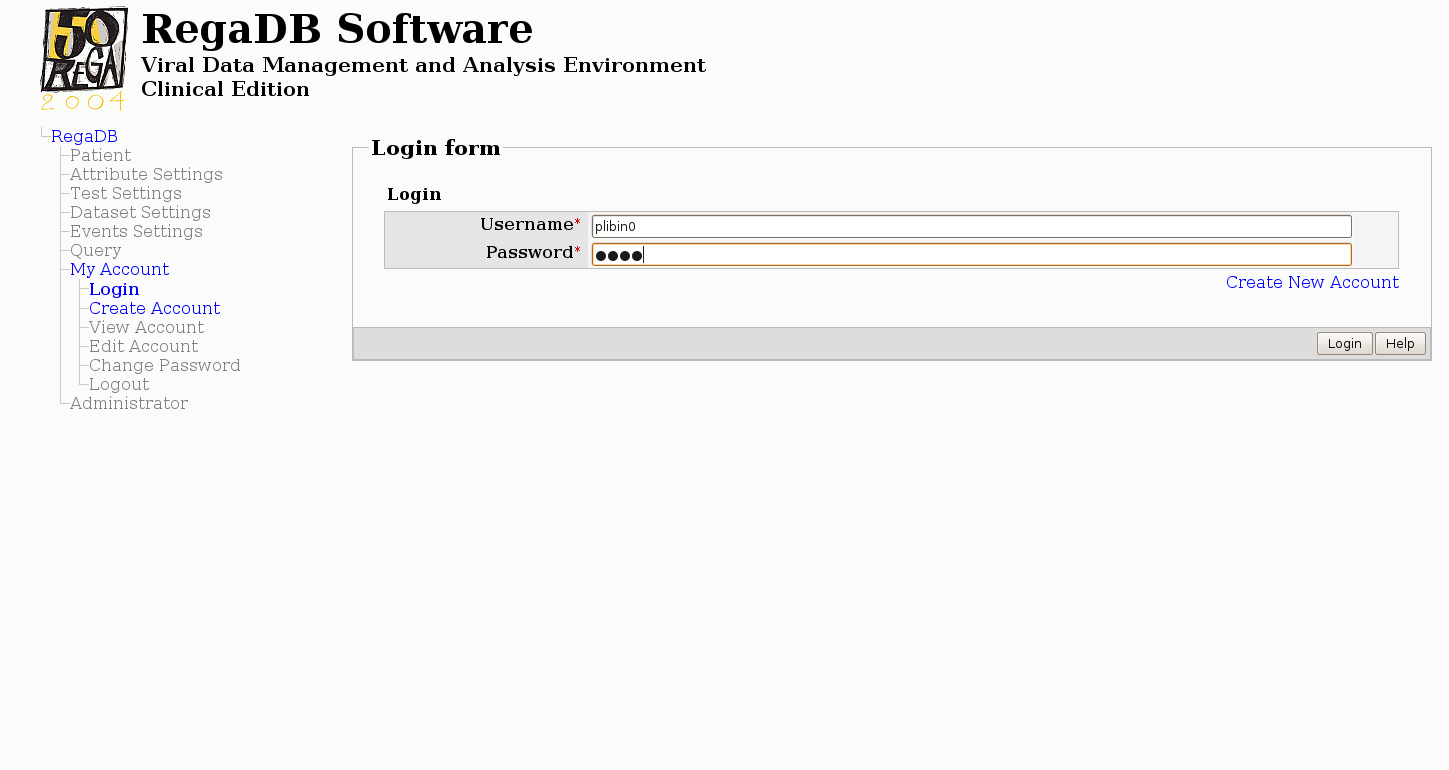
\includegraphics[width=15cm] {pics/auxilary/aux_1.png}}
\\
\vspace{0.5cm}~ \\ \centerline{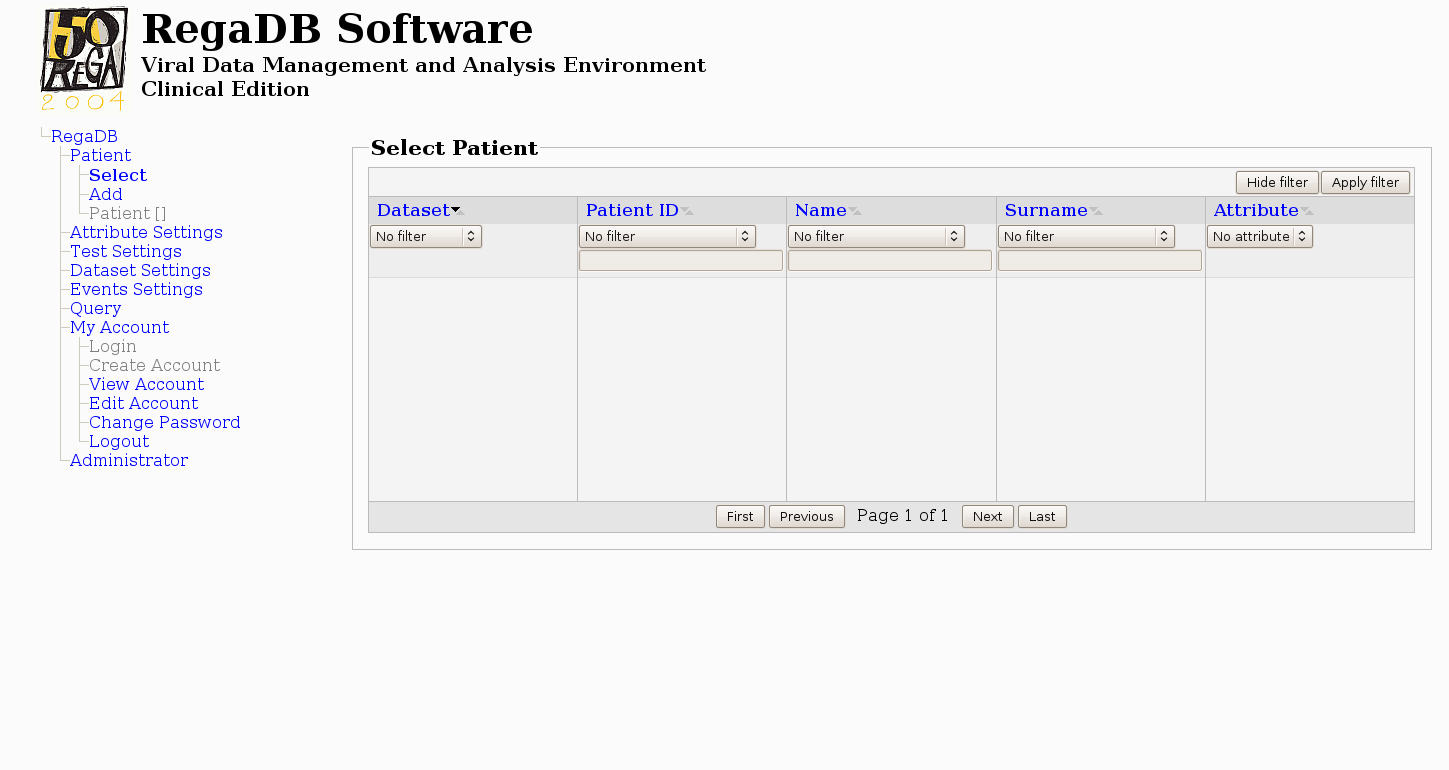
\includegraphics[width=15cm] {pics/auxilary/aux_2.png}}
\\
Navigate to the Administrator, Update from RegaDB Server page.
\\
\vspace{0.5cm}~ \\ \centerline{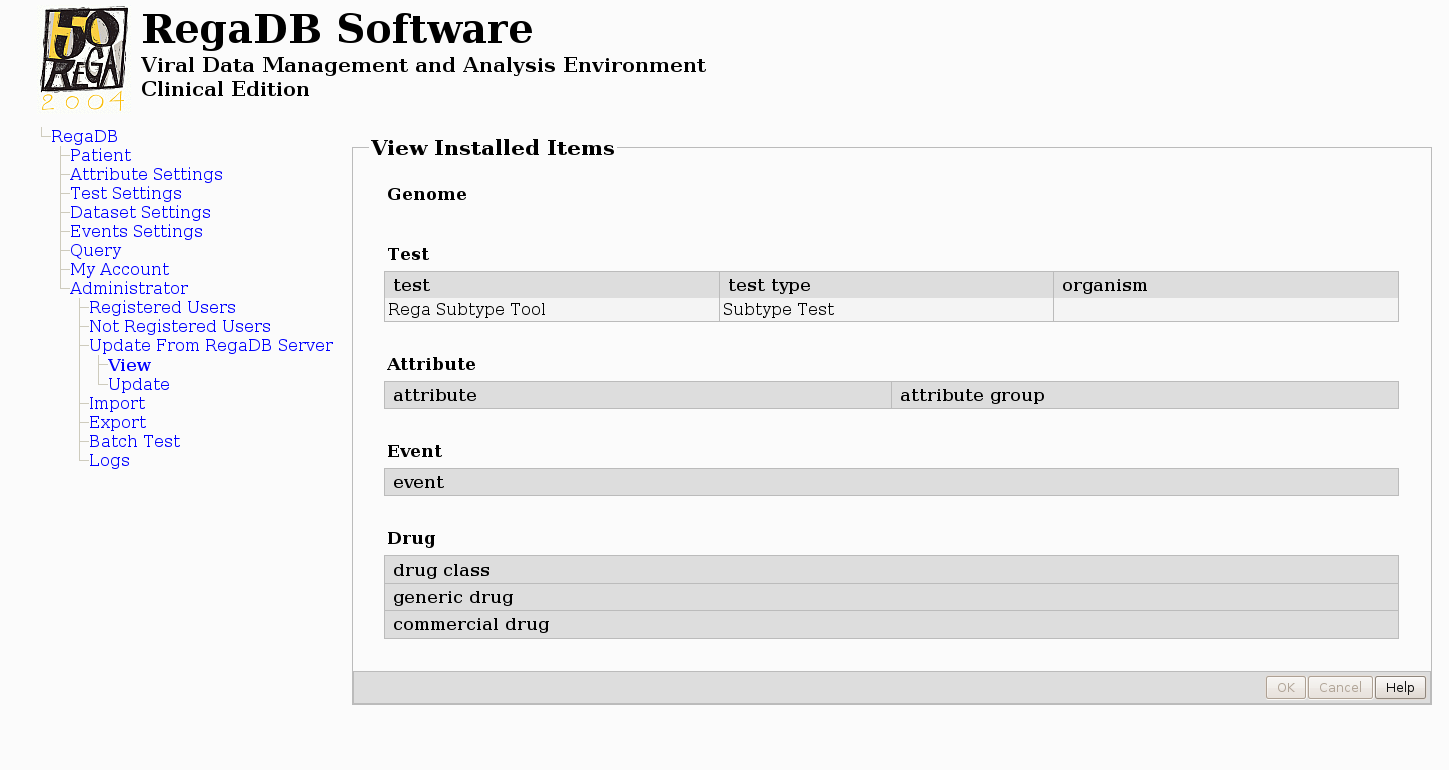
\includegraphics[width=15cm] {pics/auxilary/aux_3.png}}
\\
Click on Update, and a simulation update will be performed. This might take a few minutes, depending on your internet connection speed.
\\
\vspace{0.5cm}~ \\ \centerline{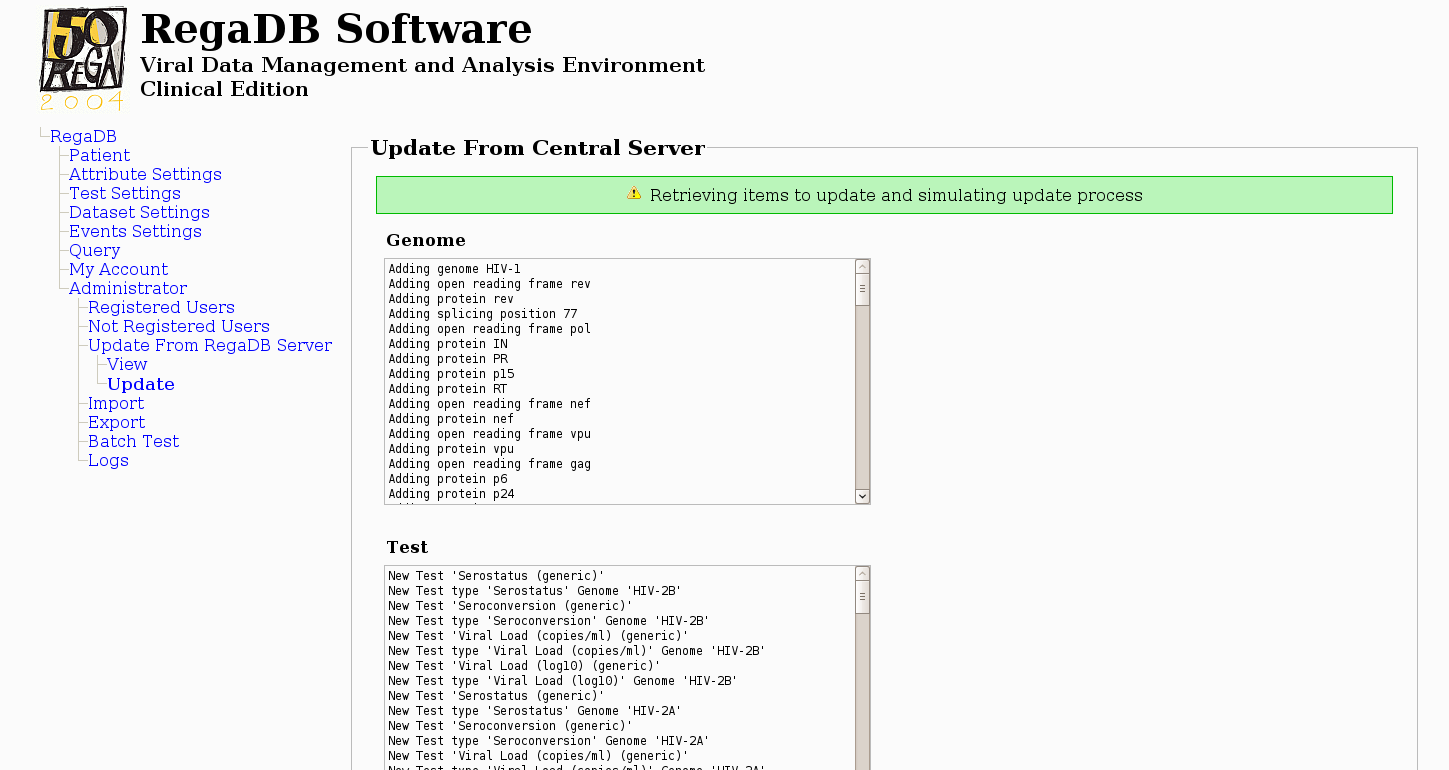
\includegraphics[width=15cm] {pics/auxilary/aux_4.png}}
\\
Click \textbf{OK} to confirm this simulation and to load the items into your local RegaDB instance. Again, this procedure might take a few minutes.
\\
\vspace{0.5cm}~ \\ \centerline{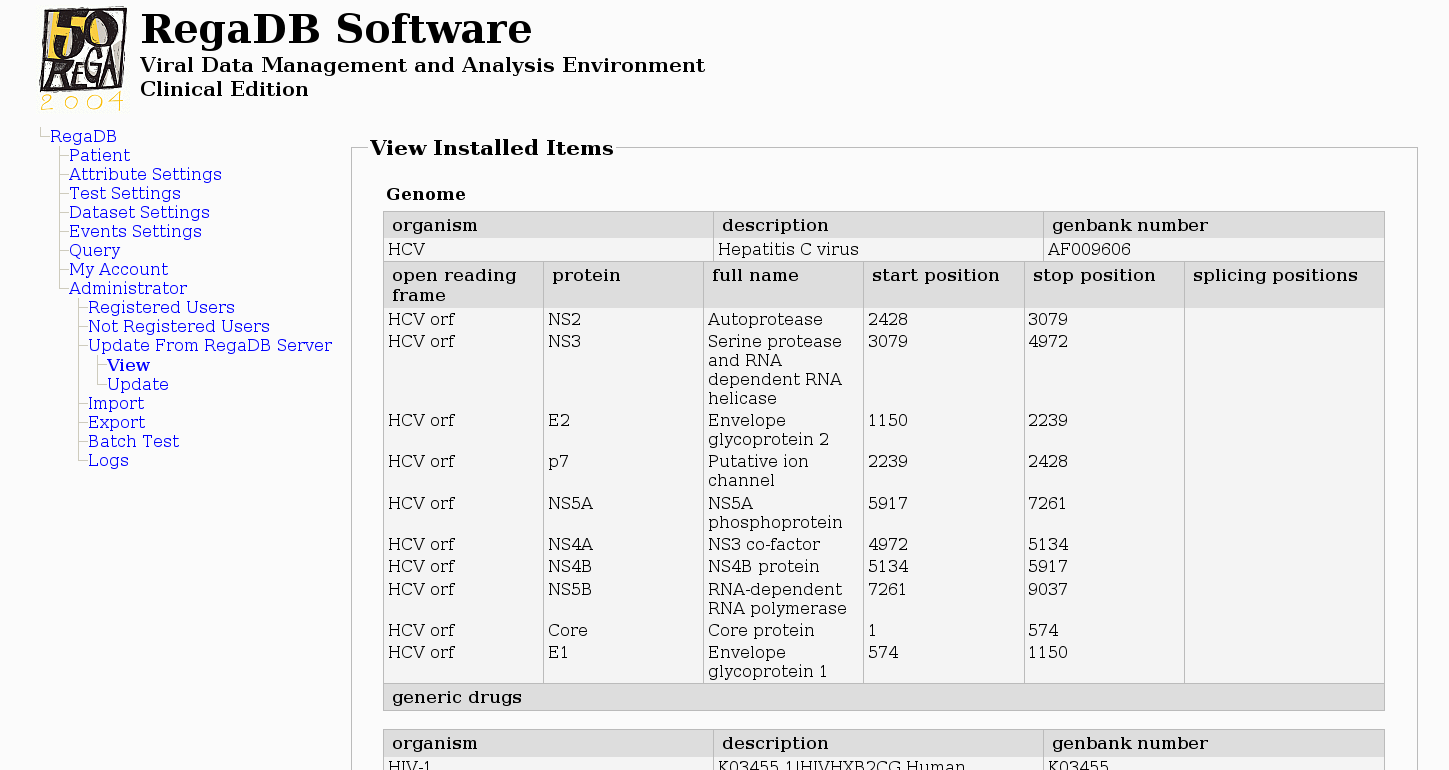
\includegraphics[width=15cm] {pics/auxilary/aux_5.png}}
\\
\section{Add a Dataset}
Navigate to the Administrator, Dataset settings menu, and add a new Dataset to the system.
